\documentclass[12pt,a4paper,ngerman]{article}

\renewcommand*\ttdefault{cmvtt}
% \usepackage{courier}
\renewcommand{\familydefault}{\ttdefault}

\usepackage[OT2,T1]{fontenc}

\renewcommand\labelitemi{---}


\usepackage{graphicx}
\usepackage[
    a4paper,
    bindingoffset=0.2cm,
    left=0.5cm,
    right=0.5cm,
    top=0.5cm,
    bottom=0.5cm,
    footskip=.25in
]{geometry}

\frenchspacing              % Better looking spacings after periods
\pagestyle{empty}           % No pagenumbers/headers/footers



\begin{document}


% %%%%%%%%%%%%%%%%%%%%%%%%%%%%%%%%%%%%%%%%%%%%%%%%%%%%%%%%%%%%%%%%%%%%%%%%%%%%%%%%%%%%
%               TITLE
% %%%%%%%%%%%%%%%%%%%%%%%%%%%%%%%%%%%%%%%%%%%%%%%%%%%%%%%%%%%%%%%%%%%%%%%%%%%%%%%%%%%%

{ \Large 9.1 }

\vspace{0.5cm}

{ \large levin eric zimmermann }

\vspace{0.25cm}

% %%%%%%%%%%%%%%%%%%%%%%%%%%%%%%%%%%%%%%%%%%%%%%%%%%%%%%%%%%%%%%%%%%%%%%%%%%%%%%%%%%%%
%               THESES
% %%%%%%%%%%%%%%%%%%%%%%%%%%%%%%%%%%%%%%%%%%%%%%%%%%%%%%%%%%%%%%%%%%%%%%%%%%%%%%%%%%%%

\begin{enumerate}

    \item{the absence of exclusion is $\infty$}

    % \item{any finite state can be described as either a finite set of all included elements or an infinite set of all excluded elements}

    \item{mystic traditions: ticket for a journey from finite state to $\infty$}

\end{enumerate}


% %%%%%%%%%%%%%%%%%%%%%%%%%%%%%%%%%%%%%%%%%%%%%%%%%%%%%%%%%%%%%%%%%%%%%%%%%%%%%%%%%%%%
%               WEIL QUOTE
% %%%%%%%%%%%%%%%%%%%%%%%%%%%%%%%%%%%%%%%%%%%%%%%%%%%%%%%%%%%%%%%%%%%%%%%%%%%%%%%%%%%%

\begin{figure}[h]
    % \hspace{-1cm}
    \begin{center}
        % \hspace{0.5cm}
        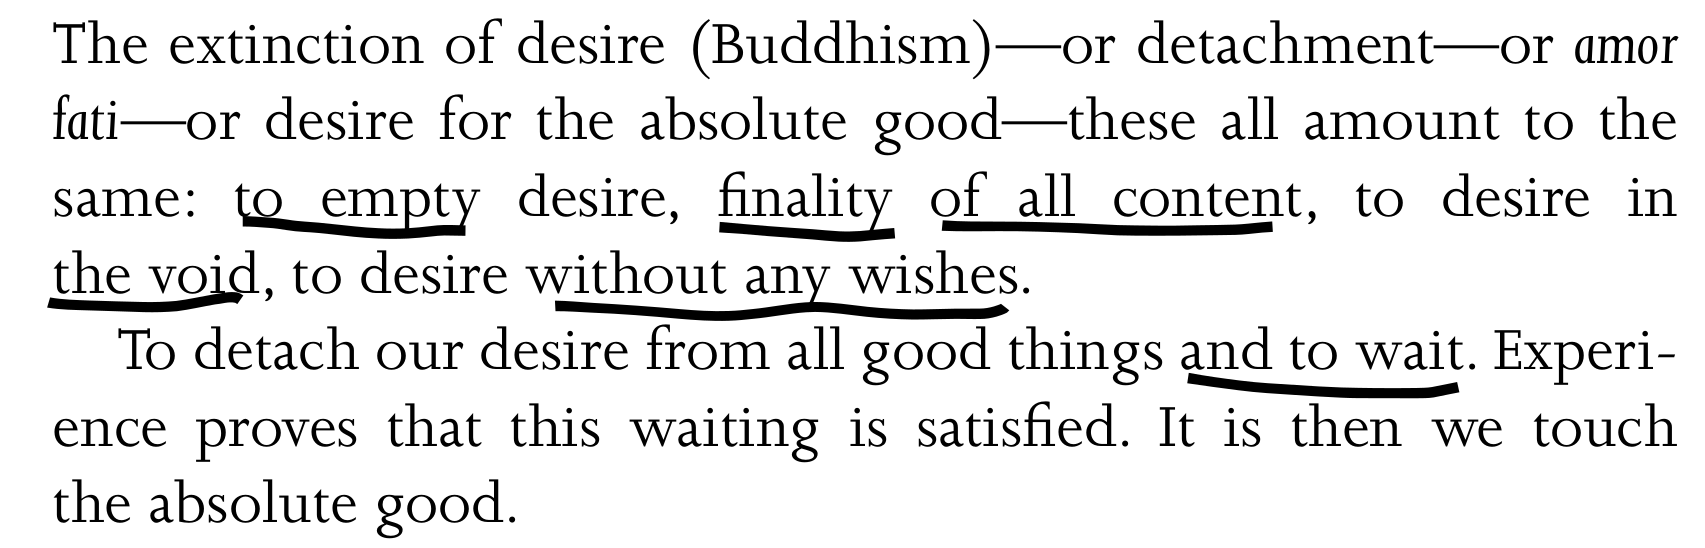
\includegraphics[scale=0.28]{pictures/weil-quote-annotated.png}
    \end{center}
    \begin{center}
        (simone weil: gravity and grace)
    \end{center}
    % \caption{%
    % }
\end{figure}


\vspace{1.5cm}


% %%%%%%%%%%%%%%%%%%%%%%%%%%%%%%%%%%%%%%%%%%%%%%%%%%%%%%%%%%%%%%%%%%%%%%%%%%%%%%%%%%%%
%               PLAYING SITUATION
% %%%%%%%%%%%%%%%%%%%%%%%%%%%%%%%%%%%%%%%%%%%%%%%%%%%%%%%%%%%%%%%%%%%%%%%%%%%%%%%%%%%%

\hspace{1.5cm} {\large full group} \hfill

\begin{itemize}

    \item{separating ourselves into independent parties}

\end{itemize}


\vspace{0.15cm}

\hspace{0.5cm} \begin{minipage}[b]{.8\textwidth}


    \footnotesize


    \begin{tabular}{l l || l l} 
        group size & division & group size & division \\ [0.5ex] 
        \hline
        3 & 3 & 10 & $4+3+3$ or $5+5$\\
        4 & 4 & 11 & $4+4+3$\\
        5 & 5 & 12 & $3+3+3+3$ or $4+4+4$ or $5+4+3$\\
        6 & $3+3$ & 13 & $4+3+3+3$ or $5+4+4$ or $5+5+3$\\
        7 & $4+3$ & 14 & $4+4+3+3$ or $5+5+4$ or $5+3+3+3$\\
        8 & $4+4$ & 15 & $4+4+4+3$ or $5+5+5$ or $5+4+3+3$\\
        9 & $3+3+3$ or $5+4$ & 16 & $4+4+4+4$ or $5+4+4+3$ or $5+5+3+3$\\
    \end{tabular}
    
\end{minipage}%

\vspace{1cm}


\hspace{1.5cm} {\large independent party} \hfill

\begin{itemize}

    \item{(communally) starting with any (commonly) agreed page}

    \item{proceeding to the next page iff everyone is finished with the current page}

    \item{(individually) starting with the pages event sequence whenever desired}

\end{itemize}

\vspace{1.5cm}


% \hspace{2cm}

% %%%%%%%%%%%%%%%%%%%%%%%%%%%%%%%%%%%%%%%%%%%%%%%%%%%%%%%%%%%%%%%%%%%%%%%%%%%%%%%%%%%%
%               HINTS
% %%%%%%%%%%%%%%%%%%%%%%%%%%%%%%%%%%%%%%%%%%%%%%%%%%%%%%%%%%%%%%%%%%%%%%%%%%%%%%%%%%%%

\newpage

\begin{minipage}[b]{.7\textwidth}

\vspace{1.5cm}
\begin{footnotesize}

    {\small (optional) hints:}

    \begin{itemize}

        \item{independent parties may or may not be displaced from each other}

        \item{membership of parties may be declared by chance operations (lottery; alphabetical order of first names)}

        \item{start page number may be gained by chance operations (using the birth date of youngest player; using dices)}

        \item{
                to reach consensus whether a page is finished or not an independent party may utilize a commonly agreed strategy %
                (having only one page on a music desk \& if everyone moved the page from the music desk to a pile on the right side, the party moves together to the next page;
                using eye contact to reach consensus)
            }

    \end{itemize}

\end{footnotesize}


\end{minipage}%



% SCORE PAGE EXAMPLE

% player | number of events to play | duration range
% 
% i       | 3                     | 10 - 20 seconds
% 
% ii      | 0                     | 30 - 100 seconds
% 
% iii     | 2                     | 10 - 90 seconds




\end{document}
